



\subsection{The L=2 case}


\begin{figure}[H]
	\centering
	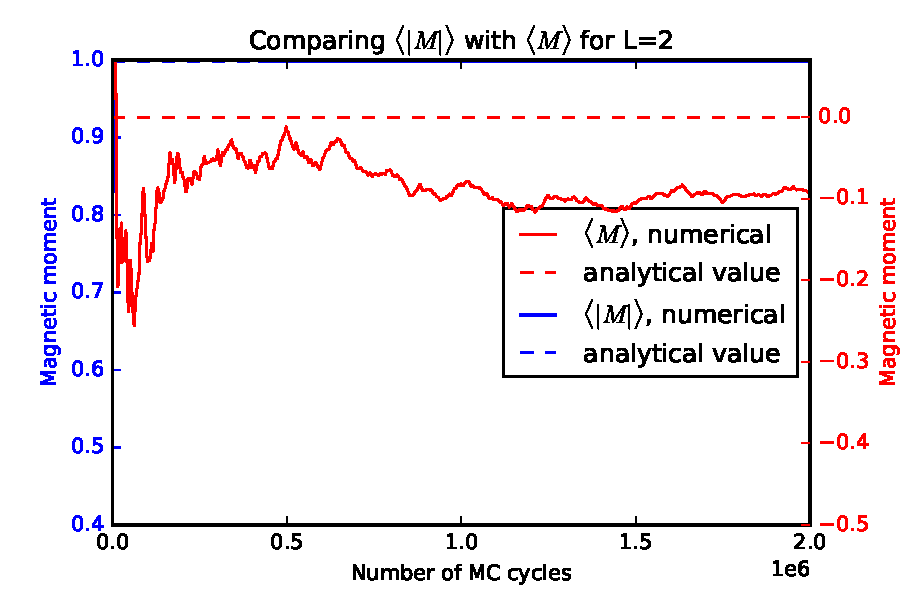
\includegraphics[width=0.7\linewidth]{../results/4b/L_2_mag_magabs}
	\caption{}
	\label{fig:l2magmagabs}
\end{figure}



	
	\begin{figure}[H]
		\begin{subfigure}[b]{0.49\textwidth}
	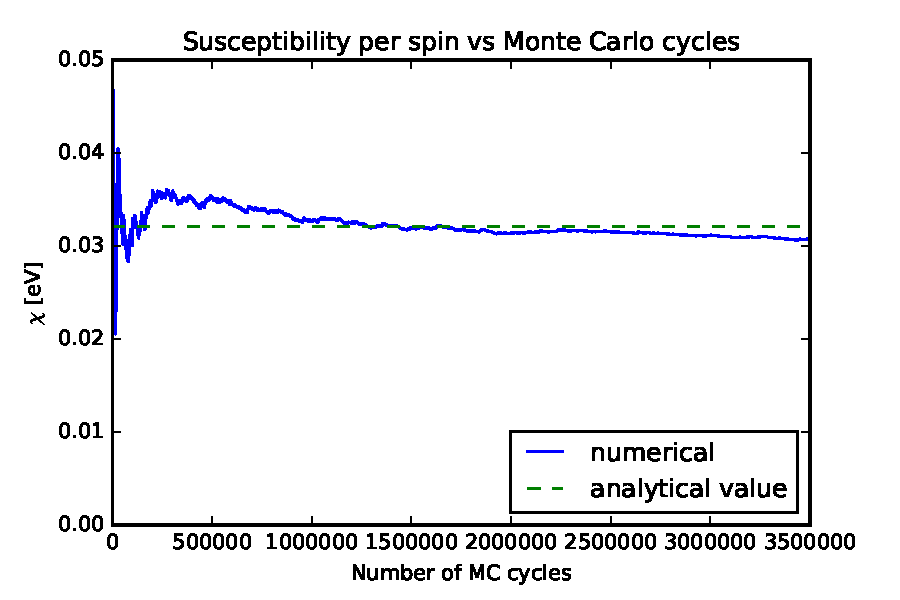
\includegraphics[width=1\linewidth]{../results/4b/L_2_susceptibility}
\caption{}
\label{fig:l2susceptibility}
		\end{subfigure}
		\hfill
		\begin{subfigure}[b]{0.49\textwidth}
		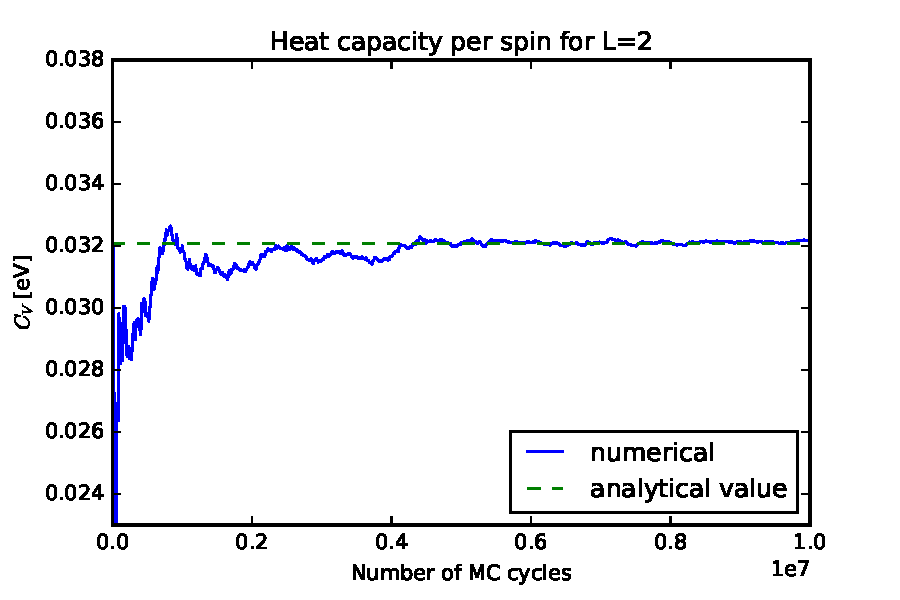
\includegraphics[width=1\linewidth]{../results/4b/L_2_heat_capasity}
\caption{}
\label{fig:l2heatcapasity}
		\end{subfigure}
		\caption{$\theta/2\theta$ scan around the (0002) peak and (0004) peak of ZnO and GaN.}
	\end{figure}

\begin{figure}[H]
	\centering
	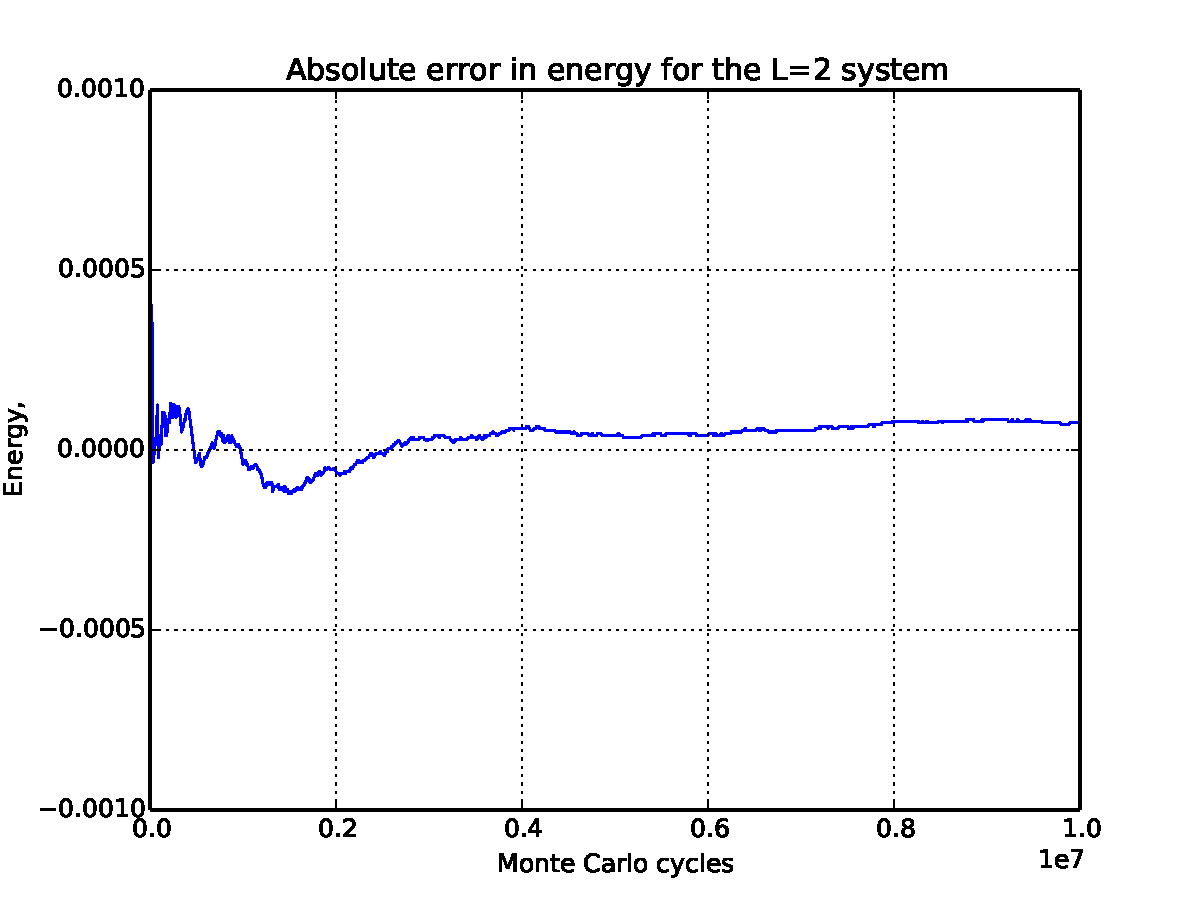
\includegraphics[width=0.7\linewidth]{../results/4b/abs_error}
	\caption{}
	\label{fig:abserror}
\end{figure}


\subsection{The L=20 system}

\subsubsection{Initial ordering of the system}

\begin{figure}[H]
	\centering
	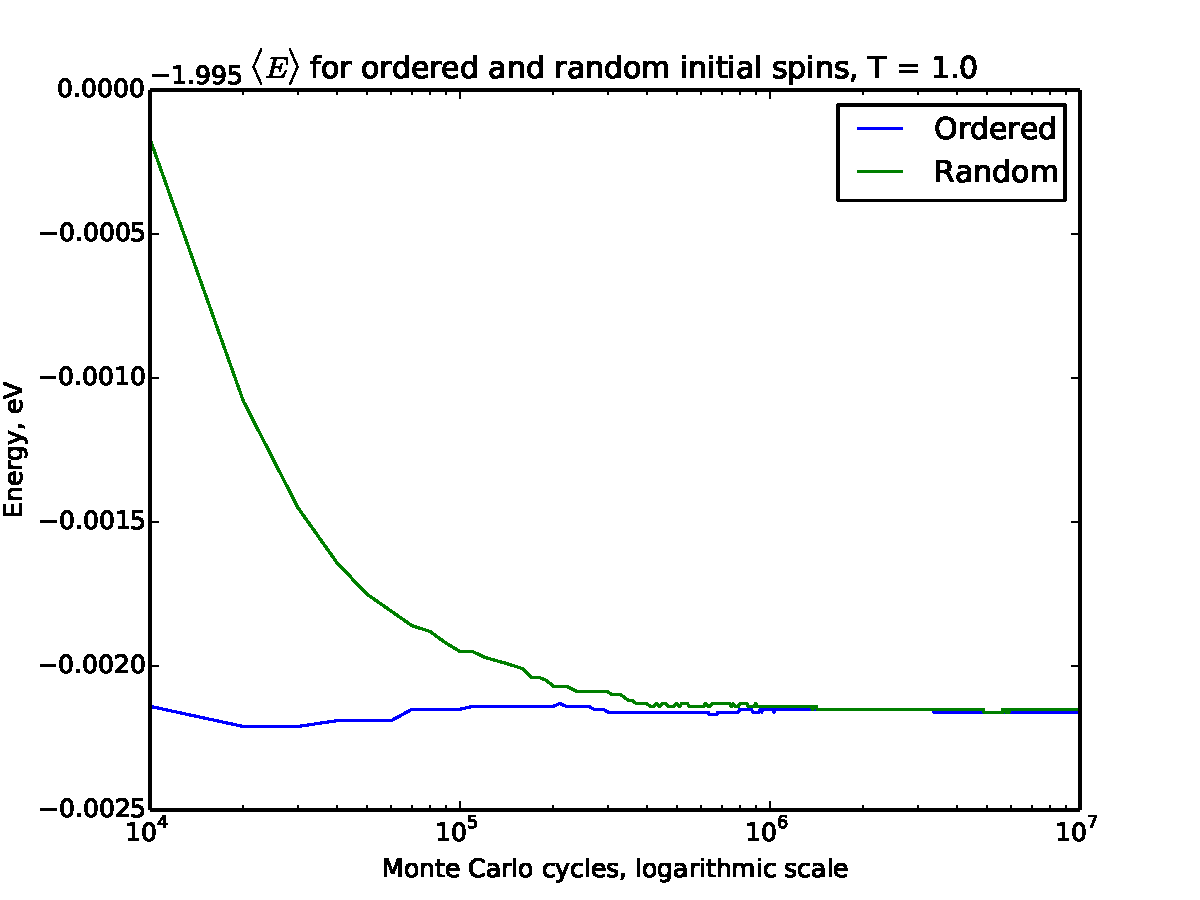
\includegraphics[width=0.7\linewidth]{../results/4c/ran_order_T1}
	\caption{}
	\label{fig:ranordert1}
\end{figure}

\begin{figure}[H]
		\centering
	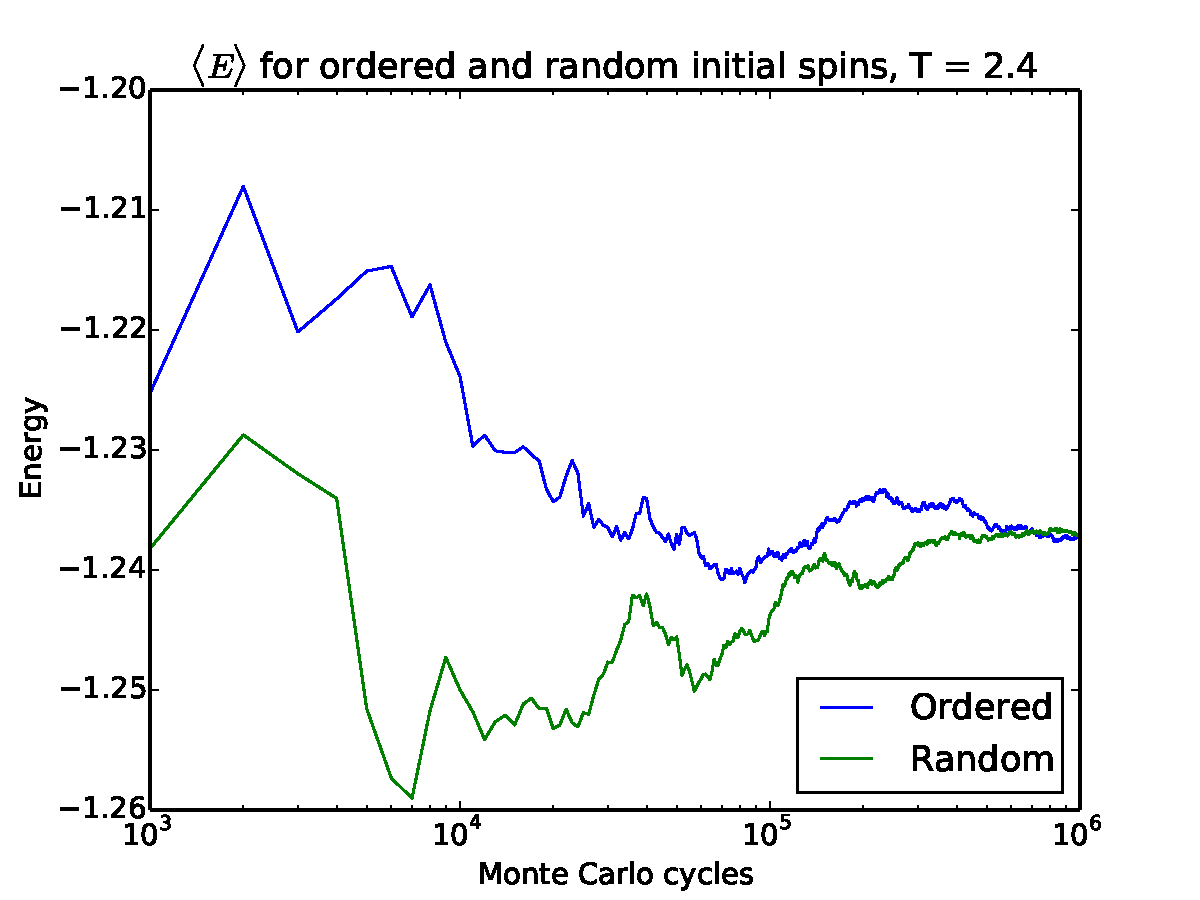
\includegraphics[width=0.7\linewidth]{../results/4c/ran_order_T2}
	\caption{}
	\label{fig:ranordert2}
\end{figure}



\begin{figure}[H]
	\centering
	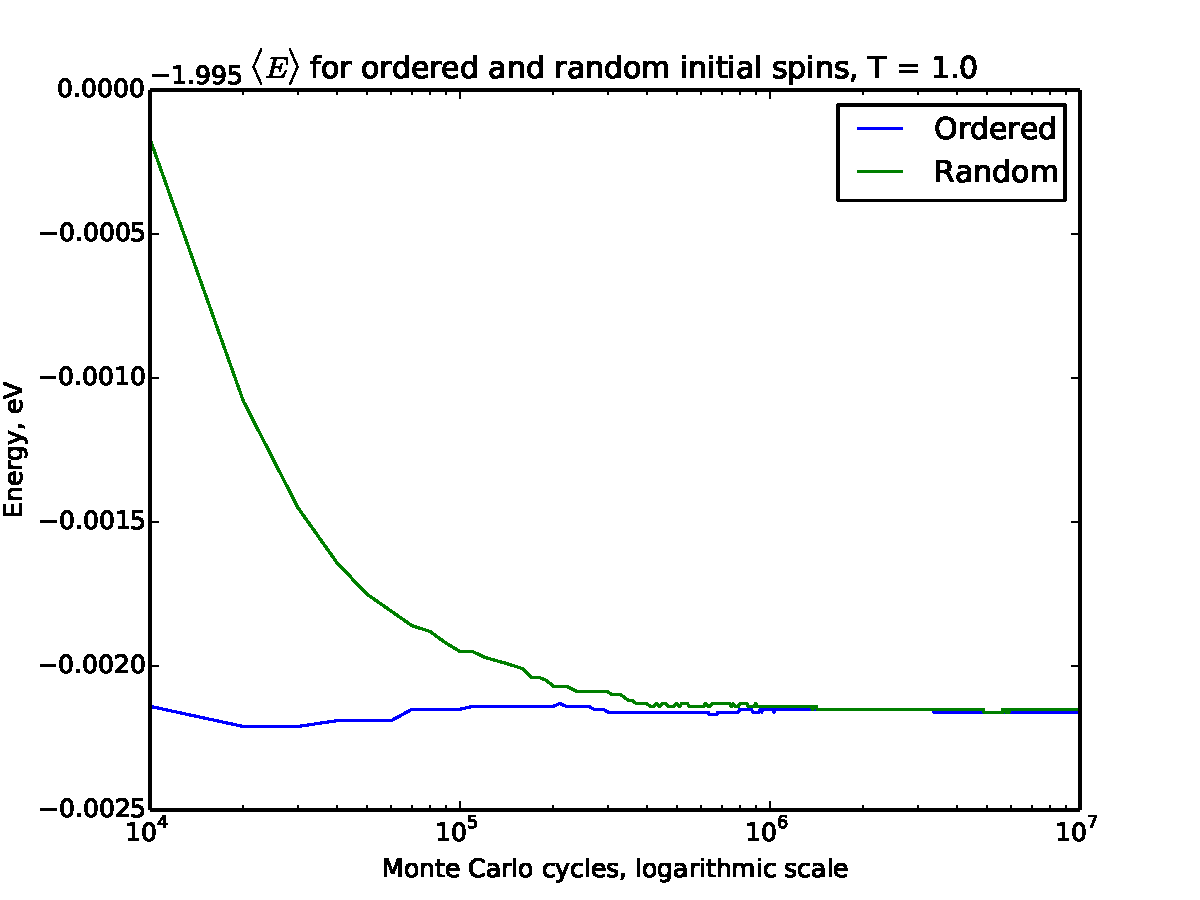
\includegraphics[width=0.7\linewidth]{../results/4c/ran_order_T1}
	\caption{}
	\label{fig:ranordert1}
\end{figure}
\begin{figure}[H]
	\centering
	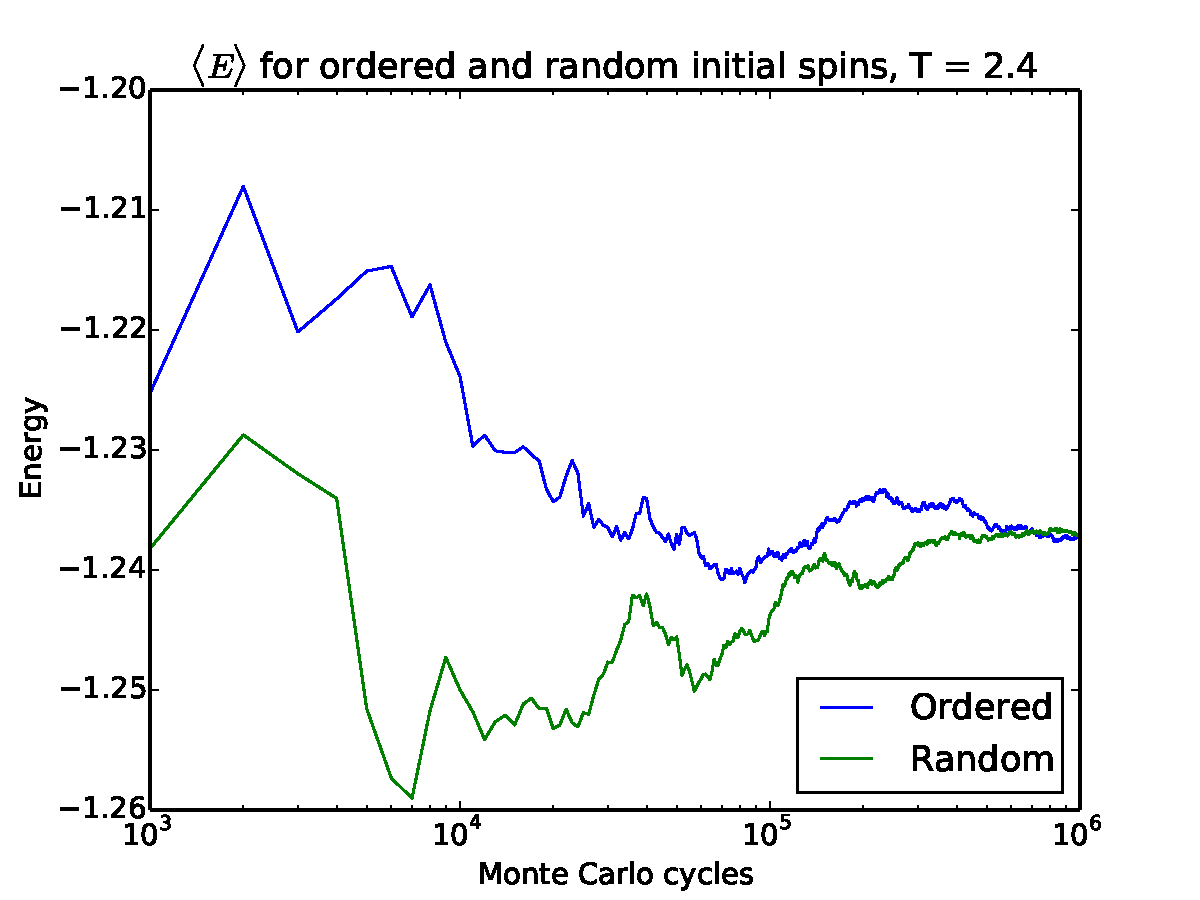
\includegraphics[width=0.7\linewidth]{../results/4c/ran_order_T2}
	\caption{}
	\label{fig:ranordert2}
\end{figure}


\begin{figure}[H]
	\centering
	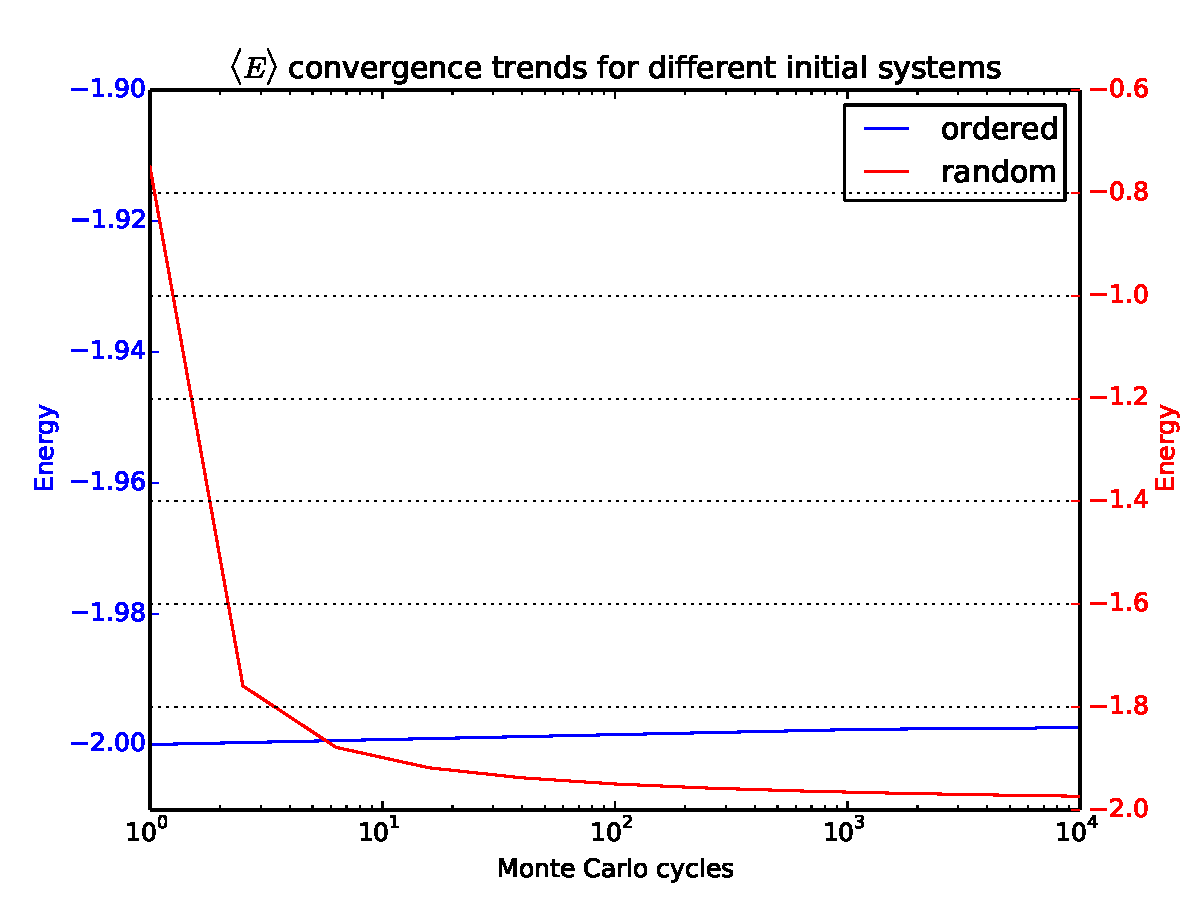
\includegraphics[width=0.7\linewidth]{../results/4c/ran_order_T1_start}
	\caption{OBS: Differnet y-axis! }
	\label{fig:ranorder_t1_start}
\end{figure}




\subsubsection{Equilibrium time  for the random L=20 system}





	\begin{figure}[H]
	\begin{subfigure}[b]{0.49\textwidth}
		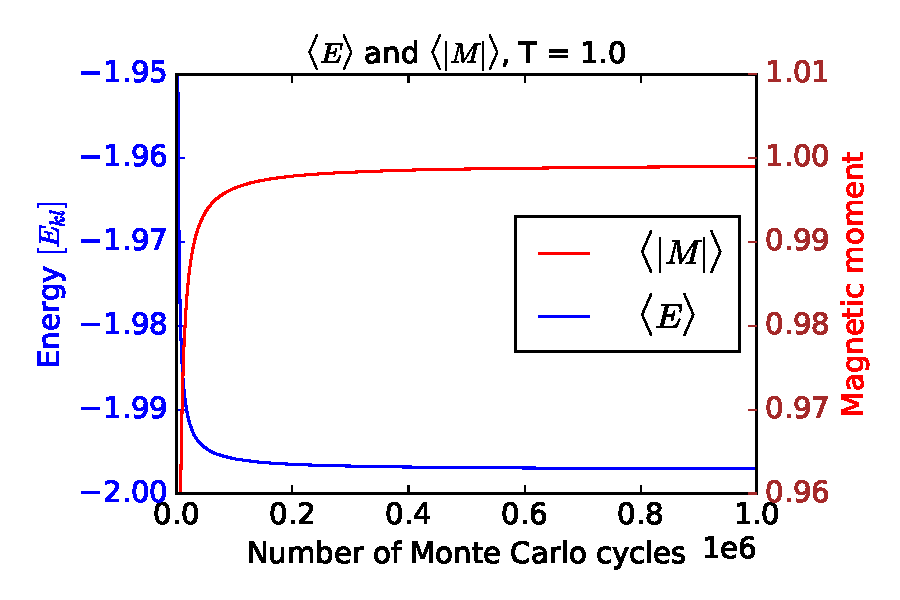
\includegraphics[width=1\linewidth]{../results/4c/En_mag_T1_0}
		\caption{}
		\label{fig:L20_mag_T_1}
	\end{subfigure}
	\hfill
	\begin{subfigure}[b]{0.49\textwidth}
		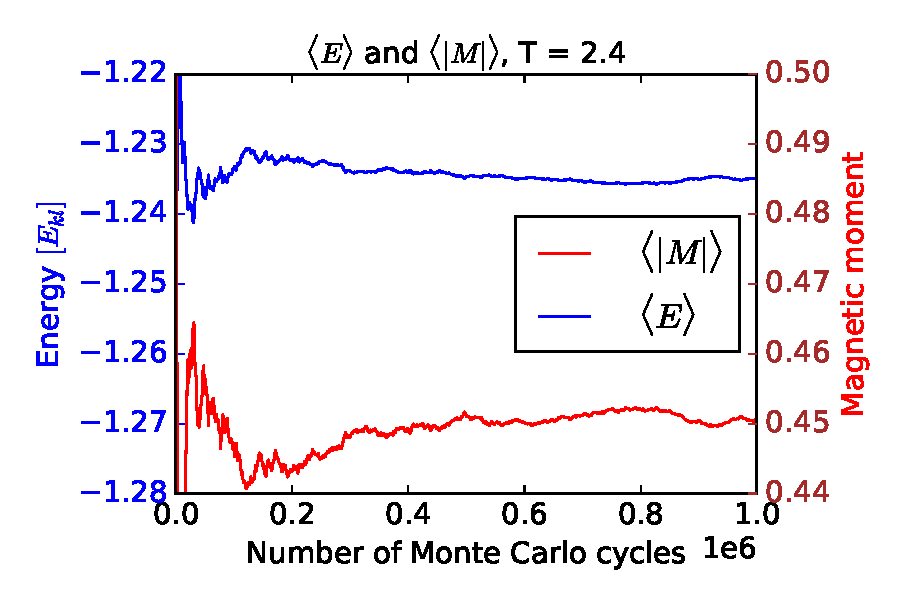
\includegraphics[width=1\linewidth]{../results/4c/En_mag_T2_4}
		\caption{}
		\label{fig:L20_mag_T_2-4}
	\end{subfigure}
	\caption{}
\end{figure}




	\begin{figure}[H]
	\begin{subfigure}[b]{0.49\textwidth}
	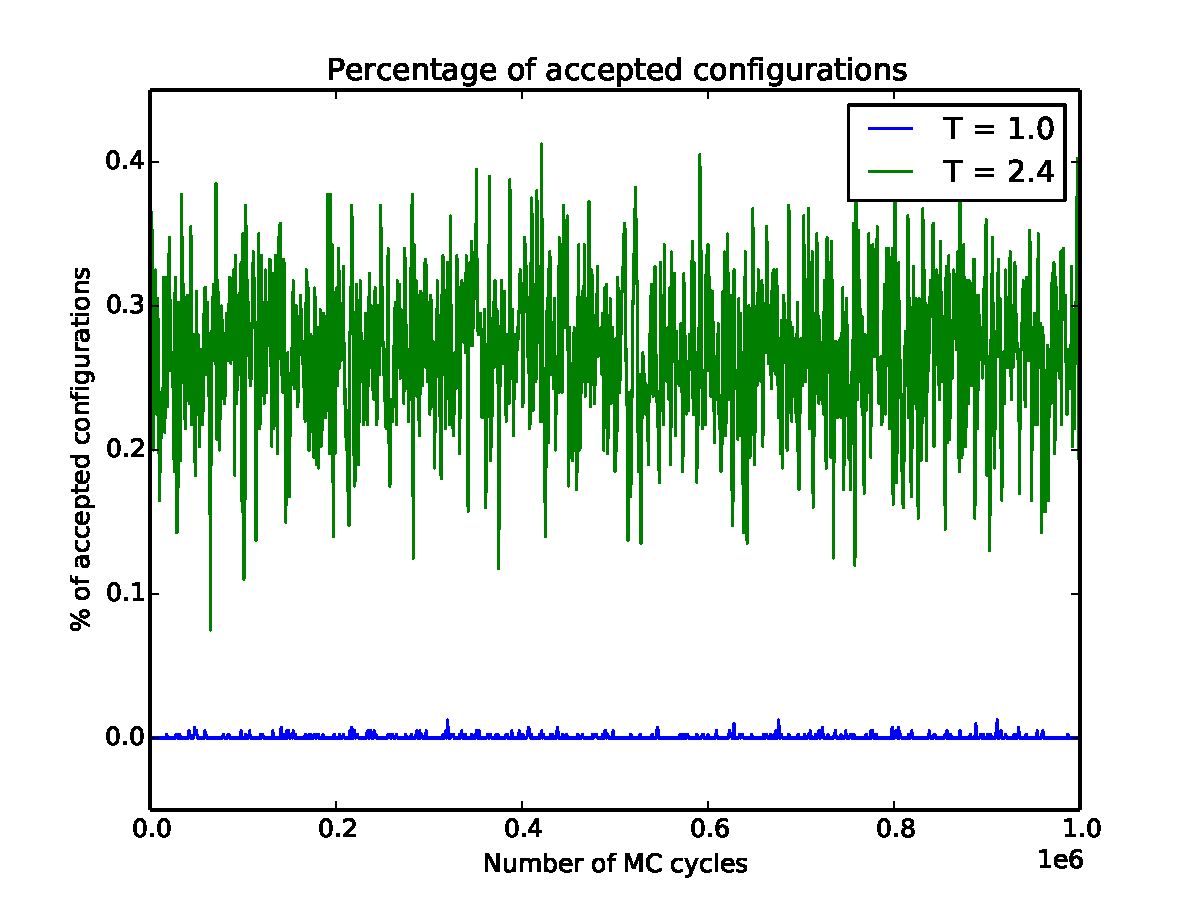
\includegraphics[width=1\linewidth]{../results/4c/L_20_accepted_configs}
\caption{}
\label{fig:l20acceptedconfigs}
	\end{subfigure}
	\hfill
	\begin{subfigure}[b]{0.49\textwidth}
	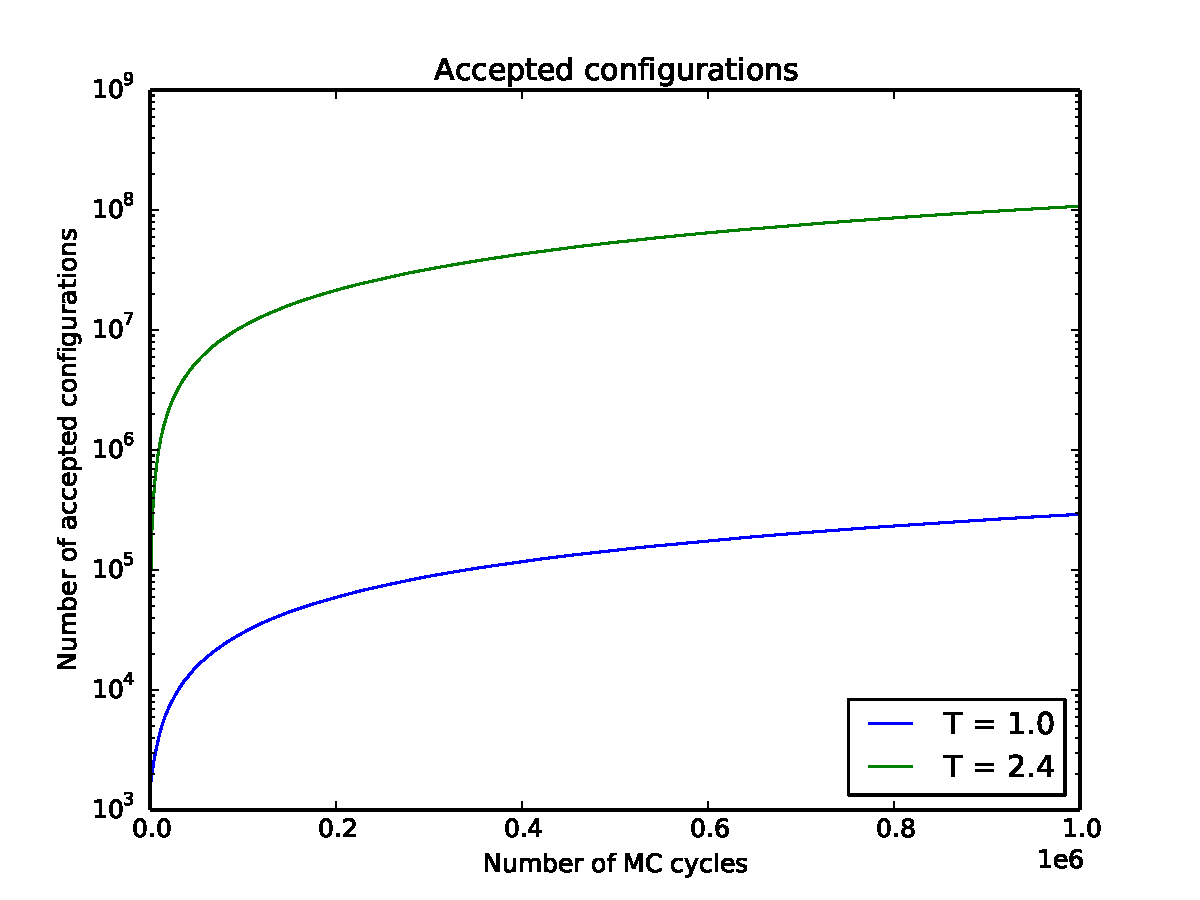
\includegraphics[width=1\linewidth]{../results/4c/L_20_accepted_configs_}
\caption{}
\label{fig:l20acceptedconfigs}
	\end{subfigure}
	\caption{}
\end{figure}











\subsubsection{Probability distrubition  for the L=20 system}



\begin{figure}[H]
	\centering
	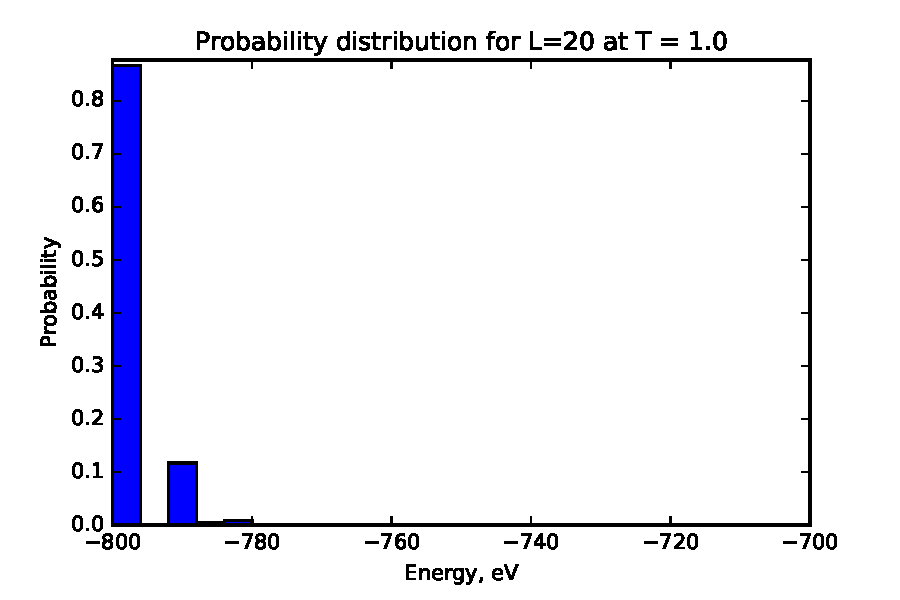
\includegraphics[width=0.7\linewidth]{../results/4d/PD_T_1MC_1e6}
	\caption{}
	\label{fig:pdt1}
\end{figure}

\begin{figure}[H]
	\centering
	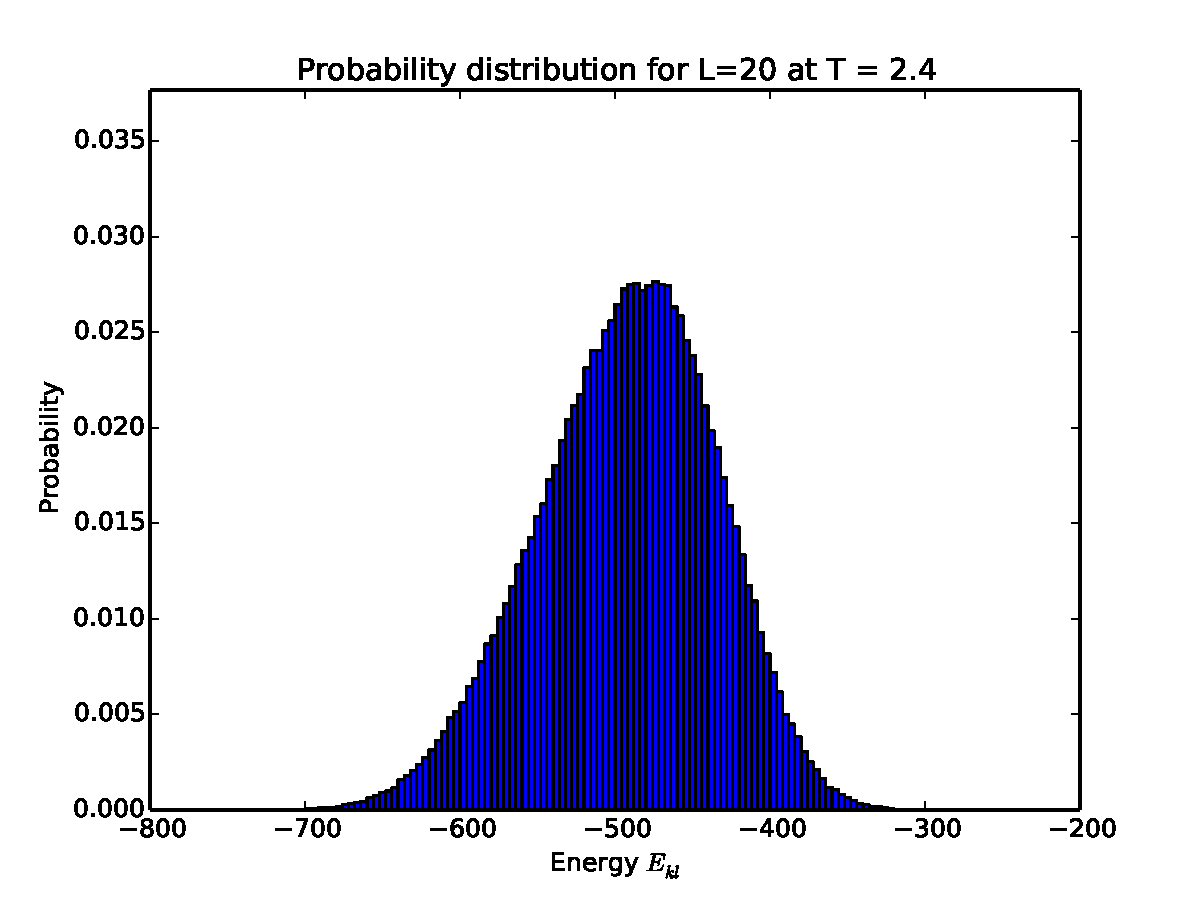
\includegraphics[width=0.7\linewidth]{../results/4d/PD_T_2MC_1e6}
	\caption{}
	\label{fig:pdt2_4}
\end{figure}



